\chapter{Introduction}
The study of analyzing human movement traces its origins back to the 19th century, notably with Charles Darwin's investigations into the connection between movement and its meaning. 
Over the years, the fields of movement analysis and non-verbal communication have made significant progress in deciphering the significance of various movements. 
They have grappled with questions like, “Do movements convey meaning in their own right?" and “How do movements convey meaning?"
Movements and non-verbal expressions hold a unique place in communication as they transcend verbal language. 
They contribute to the intricate web of conscious and subconscious communication during interactions \cite{Daly:1988},\cite{laffaye:2013}. 

However, while there is a wealth of research exploring how emotions are conveyed through facial expressions and vocal cues, the role of full-body movement and expressive gestures in this context has been somewhat overlooked until recent times.

The need for further investigation arises from the rapid advancements in technology that have made full-body real-time movement analysis more accessible and affordable. 
Humans are adept at interpreting the emotional content of non-verbal cues, which underscores the importance of studying the perception of human motion \cite{samadani:2011}. 
Emotions have been observed to manifest through posture and movements, reinforcing the idea that movement plays a crucial role in how we perceive and understand emotions.

Nonetheless, the challenge lies in determining the correct interpretation of a specific movement. 
The context in which a movement occurs is as vital as the observer's perspective. 
Movement analysis has found applications in various fields, spanning sports, the arts, and scientific research. 
One notable contribution from the realm of non-verbal communication research is the Laban Movement Analysis (LMA). 
It posits that “movement is a psycho-physical process, an outward expression of inward intent" \cite{Groff1995LabanMA}. 
LMA provides a structured notation system for examining the structure and expressiveness of movements, particularly in dance.
Within the framework of LMA, there are four distinct categories of movement elements, and one of these categories holds particular relevance to the research conducted in this thesis. 
Specifically, LMA delves into the “Body" category, which encompasses several critical aspects:
\begin{itemize}
    \item Differentiation of Body Parts and Their Interactions: LMA explores how various parts of the body differentiate and interact during movements.
    \item Description of Sequences and Simultaneous Movements: It provides a means to describe both sequences of movements and movements that occur simultaneously.  
    \item Identification of Movement Initiation Sources: Importantly, within the context of this thesis, LMA focuses on identifying the sources that initiate movements \cite{zhao2001synthesis}.
\end{itemize}
In essence, it seeks to define the \textit{origin of movement}.
    
\section{Origins and technological rise of Motion Capture}
The origin of motion capture can be traced back to the mid-20th century when rudimentary methods were employed, 
often involving manual tracking of key points on a subject's body. 
The introduction of marker-based MoCap in the 1970s marked a significant advancement. 
This technique involved attaching reflective markers to specific body points, 
which were then tracked by cameras to reconstruct the subject's movement in a digital environment. 
\begin{figure}[H]
    \centering
    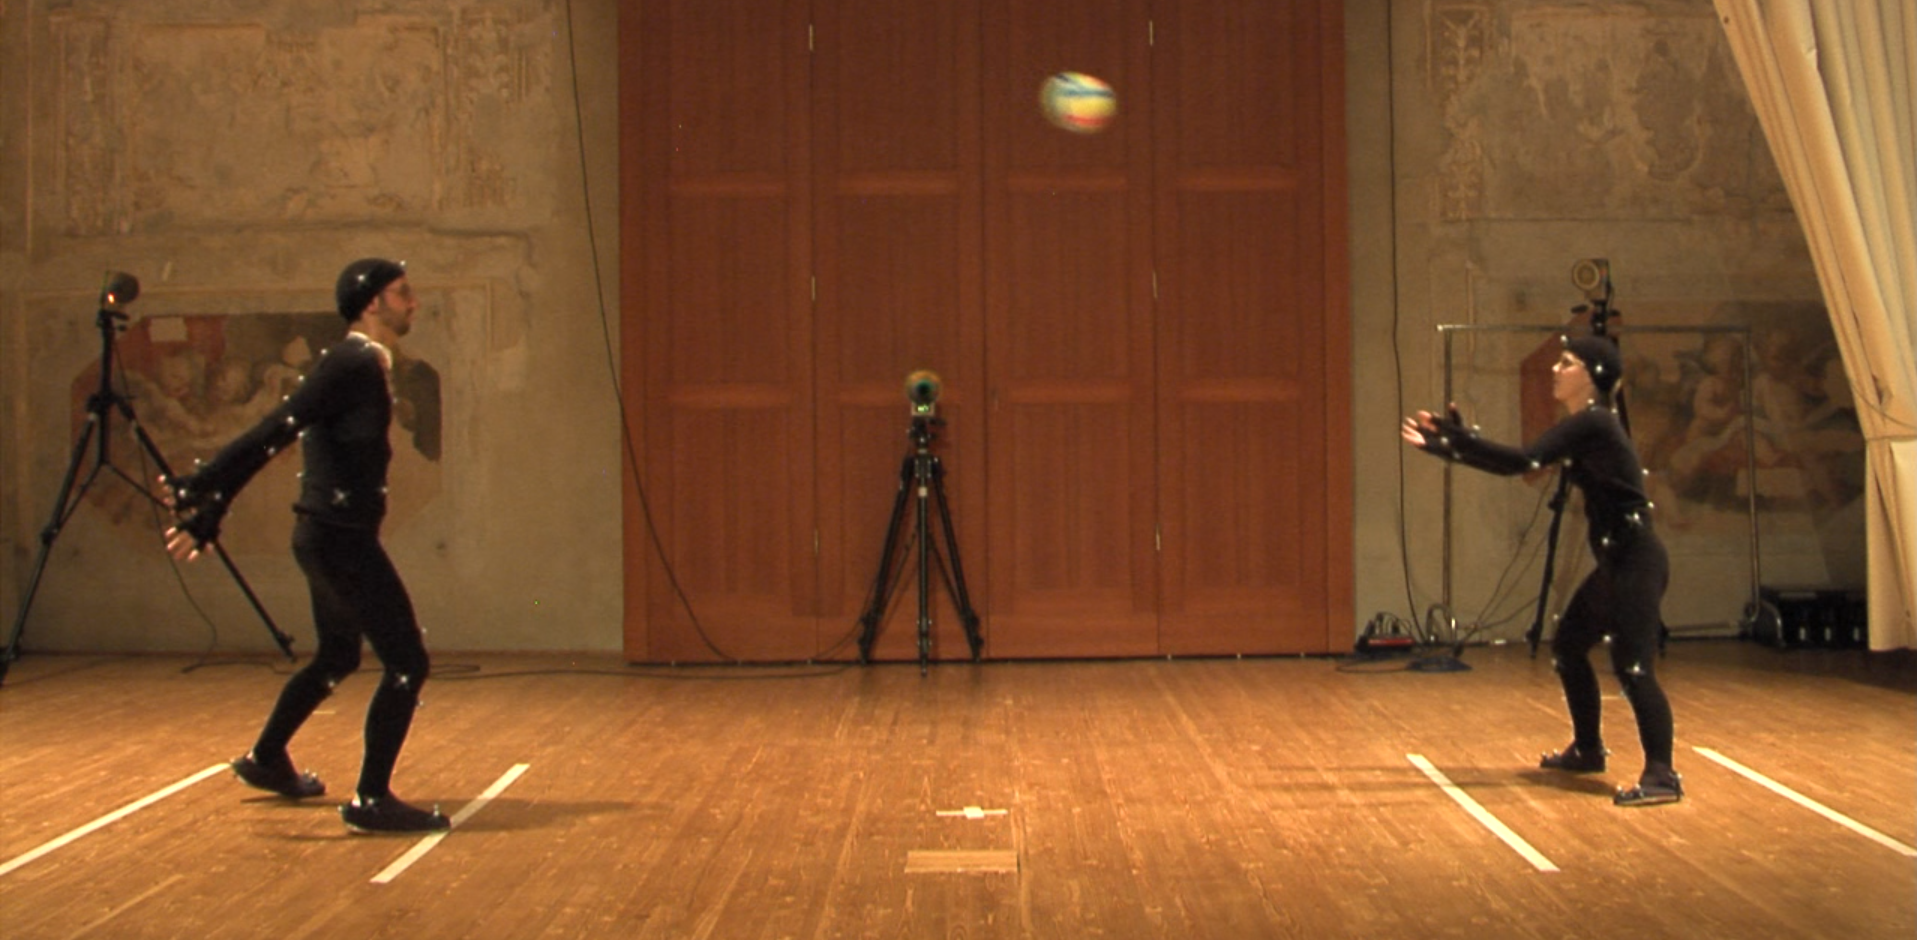
\includegraphics[width=0.8\textwidth]{graphics/bodyMarkersExampleImage.png}
    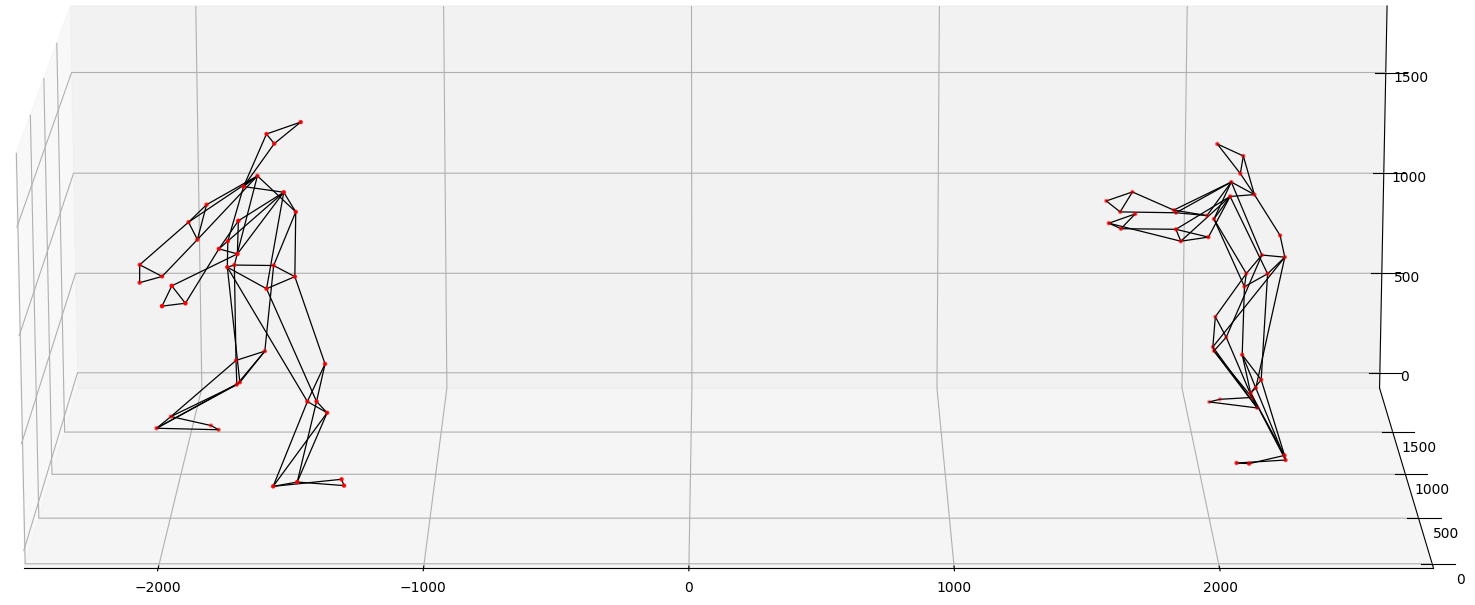
\includegraphics[width=0.8\textwidth]{graphics/bodyMarkersExampleMoCap.png}
    \caption{Video frame and MoCap scene with infrared cameras and markers}
    \label{fig:common}
\end{figure}

However, marker-based MoCap had limitations, including occlusion 
(when markers were hidden from view), inaccuracies, and the need for time-consuming calibration processes. 
These limitations led to the development of markerless MoCap technology. 
Markerless MoCap uses computer vision algorithms to track and reconstruct movement without the need for physical markers. 
This approach relies on complex algorithms that can identify and track features of the human body, 
such as joint positions and skeletal structure, from video footage.
\begin{figure}[H]
    \centering
    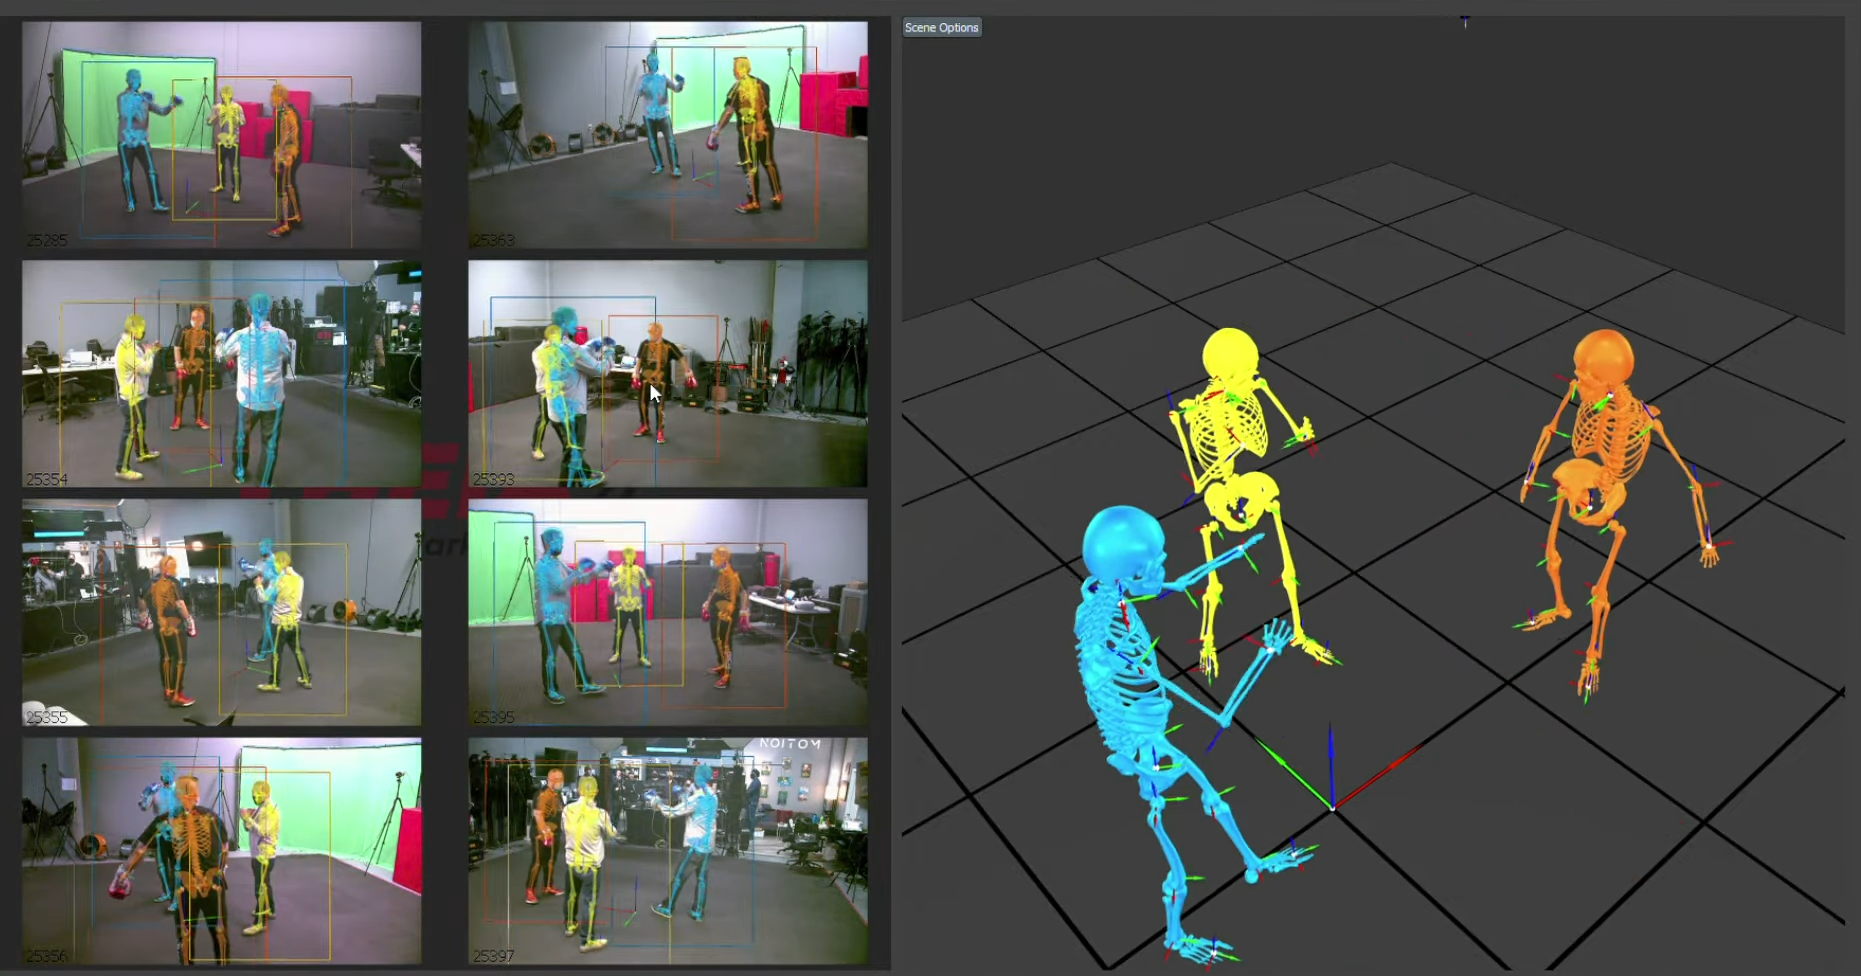
\includegraphics[width=0.8\textwidth]{graphics/MoCapMarkerlessQualisys.png}
    \caption{Markerless MoCap scene}
    \label{fig:mocap}
\end{figure}

The transition from marker-based to markerless MoCap was a result of advancements in computer vision, machine learning, and AI. 
Researchers developed algorithms capable of recognizing and tracking human motion patterns from video data, 
enabling more accurate and efficient MoCap.

The movie “Avatar," directed by James Cameron and released in December 2009, 
played a pivotal role in showcasing the potential of MoCap-based cgi applied to entertainment. 
The film featured groundbreaking visual effects, 
including the integration of live-action performances with computer-generated characters and environments. 
The production used a combination of marker-based and markerless MoCap techniques to capture the actors' 
performances and translate them into the movements of their virtual counterparts, such as the Na'vi characters.
Additionally, facial MoCap was used to capture nuanced facial expressions, enhancing the realism of the characters.
\begin{figure}[H]
    \centering
    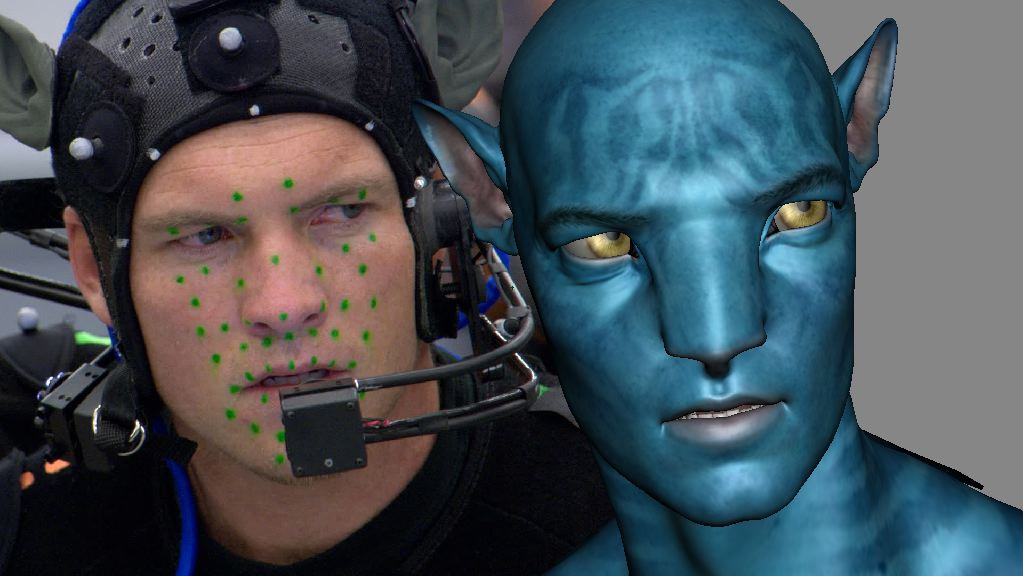
\includegraphics[width=0.8\textwidth]{graphics/avatar_markers.jpg}
    \caption[]{The actor Sam Worthington and his Na'vi Jake Sully\textsuperscript{1}}
    \label{fig:avatar}
\end{figure}

While the film's production involved a mix of traditional animation and advanced MoCap techniques, 
the seamless integration of these technologies pushed the boundaries of what was possible in terms of visual storytelling 
and character animation. 
“Avatar" demonstrated how MoCap could be used to create lifelike and emotive characters in a fantastical setting.
From marker-based recording to detection through advanced sensors and high-definition cameras, we see how technological innovations have made the MoCap process increasingly precise and detailed.

\section{Research context}
Movement is one of the first complex actions that we learn when we are born. 
It defines how we interact with the world around us. 

Studies in this field date back to Charles Darwin in 19th century with his research in the relationship 
between movement and emotions, those that are called depressing do not lead to energetic actions. 
Pain, fear, and griefs when cause complete exhaustion results in prostration, 
while excitement of the nervous system is typically expressed through frenetic and vibrant movements \cite{darwin}.  

With the Laban Movement Analysis this field reached a formalization, applied to expressive motion in dance, 
in terms of what the body is doing, interrelationships within it, quality of the movement, 
changes in physical shape and harmonic interaction of the movement with the space around. 

In general, the analysis in full-body movement spaced both retroactively and proactively as form of expression to convey emotions. 
When moving our bodies, we are not simply performing a physical shift in space, but we use it also to 
communicate affective expressions to others in a nonverbal way \cite{gelder:2009,kleinsmith:2013,karg:2013}. 
For example, the behaviour behind a “caress” can vary from care to hostility, 
if the origin of that movement is either the wrist, the shoulder or if it involves a complex 
contraction of muscle torques from the arm down to the leg. 
This interconnection between many different body parts, brought us to the leading joint hypothesis \cite{dounskaia:2010} 
which offers a novel interpretation of control of human movements that involve multiple joints 
where the central nervous system organizes the execution of the motion act, with a hierarchical process 
that originates from a leading joint and propagates back to the body part that expresses the action. 
In sports and dance, the junction between effectiveness and efficiency of a movement, while also minimizing injuries on the long-term, 
lays in the awareness and exploitation of this concept. 
In my personal experience as a martial art athlete, understanding the correct motion, 
practicing and fixing misaligned posture is the key for an efficient energy allocation and the whole performance appearance. 
For example, the correct execution of a cross punch according to the common 
knowledge within the discipline consists of a complex 
twist of the upper body with a final braking involving hips, abdominal and back muscles, 
and the rear foot’s partial rotation \cite{wasik:2013}.
\begin{figure}[H]
    \centering
    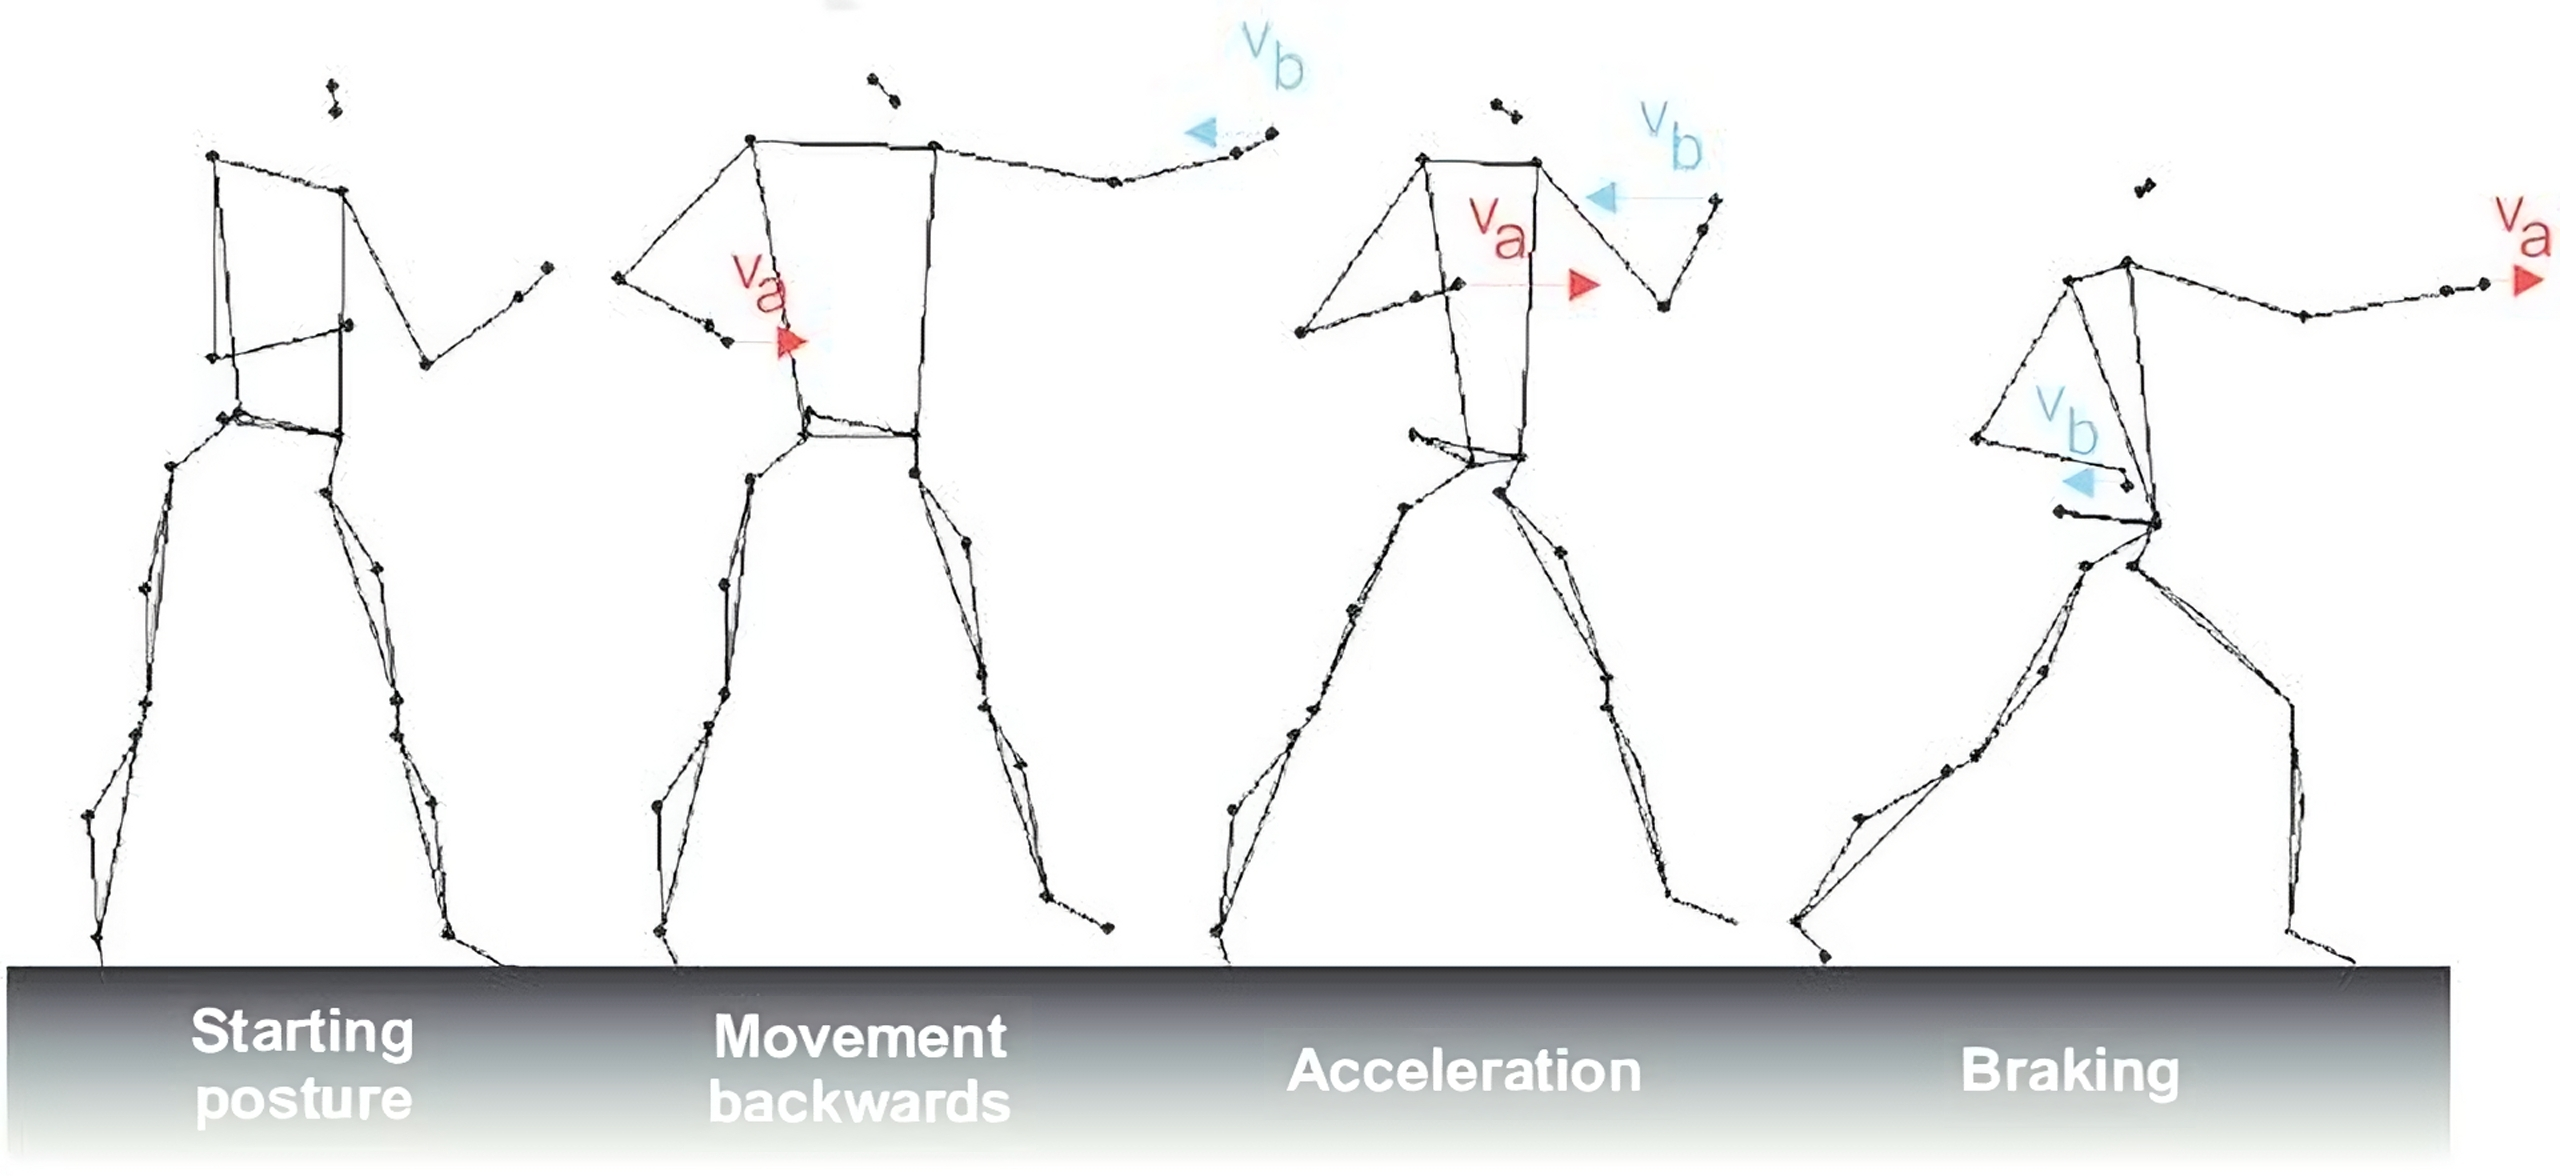
\includegraphics[width=0.8\textwidth]{graphics/Taekwon-do-joomuk-jirugi.jpeg}
    \caption{MoCap movement of the Taekwon-do joomuk jirugi}
    \label{fig:example}
\end{figure}